\documentclass[11pt]{charter}

% El títulos de la memoria, se usa en la carátula y se puede usar el cualquier lugar del documento con el comando \ttitle
\titulo{Sistema de seguimiento de procesos en rectificadora de motopartes}

% Nombre del posgrado, se usa en la carátula y se puede usar el cualquier lugar del documento con el comando \degreename
%\posgrado{Carrera de Especialización en Sistemas Embebidos} 
\posgrado{Carrera de Especialización en Internet de las Cosas} 
%\posgrado{Carrera de Especialización en Intelegencia Artificial}
%\posgrado{Maestría en Sistemas Embebidos} 
%\posgrado{Maestría en Internet de las cosas}

% Tu nombre, se puede usar el cualquier lugar del documento con el comando \authorname
\autor{Pablo Arancibia} 

% El nombre del director y co-director, se puede usar el cualquier lugar del documento con el comando \supname y \cosupname y \pertesupname y \pertecosupname
\director{Mg. Ing. Diego Fernandez}
\pertenenciaDirector{FIUBA} 
% FIXME:NO IMPLEMENTADO EL CODIRECTOR ni su pertenencia
\codirector{Ing. Miguel del Valle} % si queda vacio no se deberíá incluir 
\pertenenciaCoDirector{IUA}

% Nombre del cliente, quien va a aprobar los resultados del proyecto, se puede usar con el comando \clientename y \empclientename
\cliente{Miguel Ángel Arancibia}
\empresaCliente{ARANCIBIA Rectificaciones}

% Nombre y pertenencia de los jurados, se pueden usar el cualquier lugar del documento con el comando \jurunoname, \jurdosname y \jurtresname y \perteunoname, \pertedosname y \pertetresname.
\juradoUno{Nombre y Apellido (1)}
\pertenenciaJurUno{pertenencia (1)} 
\juradoDos{Nombre y Apellido (2)}
\pertenenciaJurDos{pertenencia (2)}
\juradoTres{Nombre y Apellido (3)}
\pertenenciaJurTres{pertenencia (3)}
 
\fechaINICIO{25 de agosto de 2020}		%Fecha de inicio de la cursada de GdP \fechaInicioName
\fechaFINALPlanificacion{22 de octubre de 2020} 	%Fecha de final de cursada de GdP
\fechaFINALTrabajo{22 de mayo de 2021}		%Fecha de defensa pública del trabajo final


\begin{document}

\maketitle
\thispagestyle{empty}
\pagebreak


\thispagestyle{empty}
{\setlength{\parskip}{0pt}
\tableofcontents{}
}
\pagebreak


\section{Registros de cambios}
\label{sec:registro}


\begin{table}[ht]
\label{tab:registro}
\centering
\begin{tabularx}{\linewidth}{@{}|c|X|c|@{}}
\hline
\rowcolor[HTML]{C0C0C0} 
Revisión & \multicolumn{1}{c|}{\cellcolor[HTML]{C0C0C0}Detalles de los cambios realizados} & Fecha      \\ \hline
1.0      & Creación del documento                                          & 27/06/2020 \\ \hline
1.1      & Entrega hasta punto 6                                           & 08/09/2020 \\ \hline
1.2      & Entrega historias de usuario										& 15/09/2020    \\ \hline
1.3	     & Entrega hasta punto 11										& 22/09/2020    \\ \hline
1.4	     & Entrega hasta punto final										& 29/09/2020    \\ \hline
%		   En varias líneas \newline
%		   A propósito                                                     & dd/mm/aaaa \\ \hline
\end{tabularx}
\end{table}

\pagebreak



\section{Acta de constitución del proyecto}
\label{sec:acta}

\begin{flushright}
Buenos Aires, \fechaInicioName
\end{flushright}

\vspace{2cm}

Por medio de la presente se acuerda con el Lic. \authorname\hspace{1px} que su Trabajo Final de la \degreename\hspace{1px} se titulará ``\ttitle'', consistirá esencialmente en el desarrollo de un sistema para seguimiento de estado de procesos en taller de rectificaciones de motopartes, y tendrá un presupuesto preliminar estimado de 600 hs de trabajo y \textcolor{red}{\$XXX}, con fecha de inicio \fechaInicioName\hspace{1px} y fecha de presentación pública \fechaFinalName.

Se adjunta a esta acta la planificación inicial.

\vfill

% Esta parte se construye sola con la información que hayan cargado en el preámbulo del documento y no debe modificarla
\begin{table}[ht]
\centering
\begin{tabular}{ccc}
\begin{tabular}[c]{@{}c@{}}Ariel Lutenberg \\ Director posgrado FIUBA\end{tabular} & \hspace{2cm} & \begin{tabular}[c]{@{}c@{}}\clientename \\ \empclientename \end{tabular} \vspace{2.5cm} \\ 
\multicolumn{3}{c}{\begin{tabular}[c]{@{}c@{}} \supname \\ Director del Trabajo Final\end{tabular}} \vspace{2.5cm} \\
%\begin{tabular}[c]{@{}c@{}}\jurunoname \\ Jurado del Trabajo Final\end{tabular}     &  & \begin{tabular}[c]{@{}c@{}}\jurdosname\\ Jurado del Trabajo Final\end{tabular}  \vspace{2.5cm}  \\
%\multicolumn{3}{c}{\begin{tabular}[c]{@{}c@{}} \jurtresname\\ Jurado del Trabajo Final\end{tabular}} \vspace{.5cm}                                                                     
\end{tabular}
\end{table}




\section{Descripción técnica-conceptual del proyecto a realizar}
\label{sec:descripcion}

\begin{consigna}{black}
El sistema a desarrollar será capaz de monitorear el estado actual de cada repuesto que se encuentre en el negocio para ser reparado.
Se desarrollará una aplicación web y una app móvil para registrar a los clientes y a cada repuesto que ingresa al taller.
Cada estado de trabajo tiene su respectivo sector (en espera, en proceso, finalizado y entregado), se utilizará un lector RFID para cada sector y una tarjeta RFID será asignada a cada repuesto ingresado.
El personal que se encargue de realizar cada trabajo de reparación será quien, a medida que va trasladando el repuesto de un sector a otro, pase la tarjeta correspondiente por cada lector RFID. 
Cada lector enviará los datos actualizados al servidor, el cual almacenará el cambio de estado en una base de datos y realizará la actualización de la información en la aplicación web.
Desde la app web/móvil se podrán visualizar todas las etapas del proceso, además los clientes podrán consultar el estado de su trabajo en tiempo real.

De esta manera se podrán mantener informados a todos los miembros de la organización sobre cuales son los procesos que se están llevando a cabo en tiempo real, tener un historial de los mismos, base de datos de clientes, informes de cantidad de trabajos por periodo de tiempo determinado, clientes frecuentes, tipos de trabajos frecuentes, entre otros.
Además cada cliente podrá consultar el estado de su trabajo, tener un historial de trabajos y recibir alertas automáticas por email o sms ante la finalización de un trabajo.

Una de las ventajas principales de este sistema es la utilización de tarjetas RFID, ya que el trabajador no necesitará ingresar datos por medio de un teclado o pantalla sino que al pasar la tarjeta por cada lector este ya enviará la información correspondiente a ser actualizada.

En la figura \ref{fig:diagBloques} se presenta el diagrama en bloques del sistema. Se puede observar como el repuesto recorre los distintos niveles del proceso representados por los lectores RFID, estos a su vez van actualizando la base de datos en el servidor y este publica los cambios en la APP para ser visualizados por quien corresponda.

\vspace{25px}

\begin{figure}[htpb]
\centering 
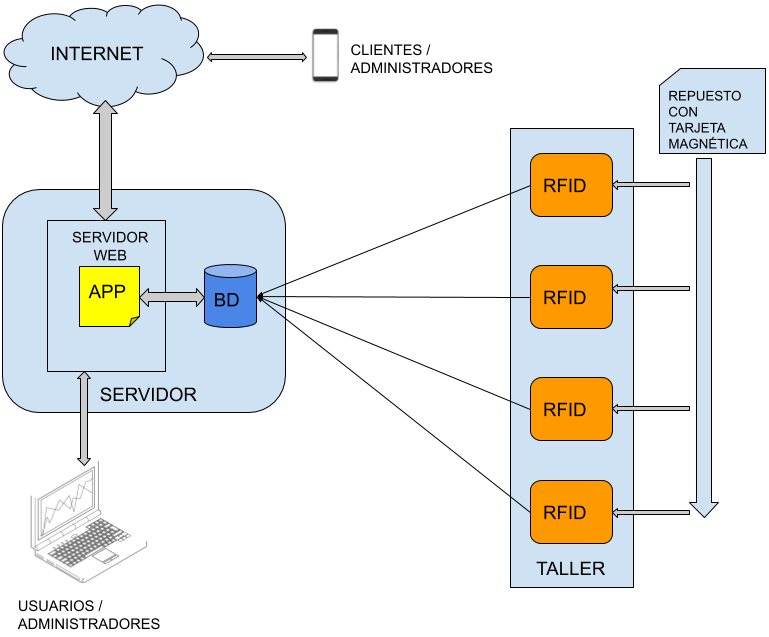
\includegraphics[width=.9\textwidth]{./Figuras/diagBloques.png}
\caption{Diagrama en bloques del sistema}
\label{fig:diagBloques}
\end{figure}

\vspace{25px}

\end{consigna}


\section{Identificación y análisis de los interesados}
\label{sec:interesados}

\begin{consigna}{black} 
%Nota: (borrar esto y todas las consignas en color rojo antes de entregar este documento).
 
%Es inusual que una misma persona esté en más de un rol, incluso en proyectos chicos.
 
%Si se considera que una persona cumple dos o más roles, entonces sólo dejarla en el rol más importante. Por ejemplo:



\begin{table}[ht]
%\caption{Identificación de los interesados}
%\label{tab:interesados}
\begin{tabularx}{\linewidth}{@{}|l|X|X|l|@{}}
\hline
\rowcolor[HTML]{C0C0C0} 
Rol           & Nombre y Apellido & Organización 	& Puesto 	\\ \hline
%Auspiciante   &                   &              	&        	\\ \hline
Cliente       & \clientename      &\empclientename	&        	\\ \hline
%Impulsor      &                   &              	&        	\\ \hline
Responsable   & \authorname       & FIUBA        	& Alumno 	\\ \hline
Colaboradores &  Miguel del Valle & Fuerza Aérea   	& Colaboración en hardware\\ \hline
Orientador    & \supname	      & \pertesupname 	& Director	Trabajo final \\ \hline
%Equipo        & miembro1 \newline 
%				miembro2          &              	&        	\\ \hline
%Opositores    &                   &              	&        	\\ \hline
Usuario final & --------------  &\empclientename &----------- \\ \hline
\end{tabularx}
\end{table}

%El Director suele ser uno de los Orientadores.

%No dejar celdas vacías; si no hay nada que poner en una celda colocar un signo ``-''.

%No dejar filas vacías; si no hay nada que poner en una fila entonces eliminarla.

%Sería deseable listar a continuación de la tabla las principales características de cada interesado.
 
%Por ejemplo:
\begin{itemize}
%\item Auspiciante: es riguroso y exigente con la rendición de gastos. Tener mucho cuidado con esto.
\item Colaborador: se deberá contactar de manera online siempre ya que reside en otra provincia.
%\item Orientador: María Gómez, nos va a poder ayudar mucho con la gestión de impuestos.
\end{itemize}

\end{consigna}



\section{1. Propósito del proyecto}
\label{sec:proposito}

\begin{consigna}{black}
El propósito de este proyecto es brindar una solución para la supervisión de estados de procesos en negocio familiar de reparación de repuestos. 

\end{consigna}

\section{2. Alcance del proyecto}
\label{sec:alcance}

\begin{consigna}{black}

El proyecto incluye:
\begin{itemize}
\item App Web
\item App Móvil
\item Servidor web
\item Servidor - Procesador
\item Base de Datos
\item Lectores RFID
\item Tarjetas magnéticas (50 unidades)
\item Instalación y configuración de todo el sistema
\item Capacitación
\item Manuales
\item 3 meses de garantía de mantenimiento
\end{itemize}

El proyecto no incluye:
\begin{itemize}
\item Dispositivos cliente: CPU, Celulares, etc.
\item Servicio de Internet
\item UPS o estabilizadores de tensión
\end{itemize}

\end{consigna}


\section{3. Supuestos del proyecto}
\label{sec:supuestos}

\begin{consigna}{black}

Para el desarrollo del presente proyecto se supone que:
\begin{itemize}
\item El cliente cuenta con conexión a Internet en la organización
\item Los empleados de mostrador tienen conocimientos mínimos de PC
\item El cliente autorizará el ingreso a la organización durante el desarrollo para la realización de pruebas iniciales.

\end{itemize}


\end{consigna}

\section{4. Requerimientos de Software}
\label{sec:requerimientos}

\begin{consigna}{black}
%Los requerimientos deben numerarse y de ser posible agruparlos por afinidad:

\begin{enumerate}
\item Grupo de requerimientos asociados con el Servidor:
	\begin{enumerate}
	\item Comunicación websocket con Esp32 (lectores RFID)
	\item Almacenamiento de base de datos (MySql,MariaDB o PostgreSql)
	\item Procesamiento en lenguaje de nivel medio (Python)
	\item Tecnologías Rest para comunicación con los demás servicios.
	\\\\ Prioridad del requerimiento: alta.
	\end{enumerate}
\item Grupo de requerimientos asociados con Aplicación Web
	\begin{enumerate}
	\item Registro de repuestos entrantes
	\item Actualización inmediata de estados de procesos
	\item ABM de clientes
	\item Búsqueda avanzada: por fecha, por cliente, por estado (para usuarios y administradores)
	\item Búsqueda de repuestos por id (para clientes) sin necesidad de acceso con usuario y contraseña.
	\item Roles: Usuario, Administrador, Cliente. Con nombre de usuario y contraseña excepto clientes.
	\item Diseño web adaptable (responsive design) y amigable.
	\\\\ Prioridad del requerimiento: alta.
	\end{enumerate}
\item Grupo de requerimientos asociados con Aplicación Móvil
	\begin{enumerate}
	\item Actualización inmediata de estados de procesos
	\item Búsqueda avanzada: por fecha, por cliente, por estado (para usuarios y administradores)
	\item Búsqueda de repuestos por id (para clientes) sin necesidad de acceso con usuario y contraseña.
	\item Roles: Usuario, Administrador, Cliente. Con nombre de usuario y contraseña excepto clientes.
	\item Diseño amigable.
	\\\\ Prioridad del requerimiento: media.
	\end{enumerate}
\end{enumerate}

%Leyendo los requerimientos se debe poder interpretar cómo será el proyecto y su funcionalidad.

%De ser posible indicar cómo se obtuvieron cada uno de los requerimientos 

%Indicar claramente cuál es la prioridad entre los distintos requerimientos. 

%No olvidarse de que los requerimientos incluyen a las regulaciones y normas vigentes!!!

%Y al escribirlos seguir las siguientes reglas:
%\begin{itemize}
%\item Ser breve y conciso (nadie lee cosas largas). 
%\item Ser específico: no dejar lugar a confusiones.
%\item Expresar los requerimientos en términos que sean cuantificables y medibles.
%\end{itemize}

\end{consigna}

\section{Historias de usuarios (\textit{Product backlog})}
\label{sec:backlog}

%\begin{consigna}{red}
%Descripción: En esta sección se deben incluir las historias de usuarios y su ponderación (\textit{history points}). Recordar que las historias de usuarios son descripciones cortas y simples de una característica contada desde la perspectiva de la persona que desea la nueva capacidad, generalmente un usuario o cliente del sistema. La ponderación es un número entero que representa el tamaño de la historia comparada con otras historias de similar tipo.
%\end{consigna}

\begin{consigna}{black}

Criterio de ponderación: se utilizó la serie de Fibonacci para establecer los puntos.  

Historia 1: como jefe de taller quiero tener una lista que se actualice inmediatamente cuando un repuesto ingresa a la empresa, con el objetivo de establecer prioridades de servicio.
\\Ponderación: 13 puntos.

Historia 2: como encargada de redes sociales y telefonista necesito tener actualizado y a mano el estado de trabajos para informar a los clientes ante una consulta.
\\Ponderación: 34 puntos.

Historia 3: como personal del mostrador me gustaría tener una Cartera de clientes digitalizada para no tener que cargar una y otra vez a los mismos clientes cada vez que traen un repuesto a reparar.
\\Ponderación: 13 puntos.

Historia 4: como contadora quiero tener un balance de trabajos diarios, semanales y mensuales que se genere de manera automática para no tener que demorar en hacer conteos de tickets como se realiza actualmente, además se reducirían las posibilidades de cometer errores en los cálculos.
\\Ponderación: 21 puntos.

Historia 5: como cliente frecuente me interesaría poder revisar el estado de mis trabajos desde mi celular para saber cuando tengo que venir a buscarlos sin necesidad de realizar una llamada telefónica.
\\Ponderación: 34 puntos.

Historia 6: como empleado de taller quiero que exista una lista de estados de trabajos de manera que no tenga yo que interrumpir mis tareas para buscar un repuesto específico cada vez que hay que informar sobre los mismos ante una consulta.
\\Ponderación: 8 puntos.


\end{consigna}

\section{5. Entregables principales del proyecto}
\label{sec:entregables}

\begin{consigna}{black}
Se entregarán: 
\begin{itemize}
\item Manual de uso
\item Diagrama de instalación
\item Informe final

\end{itemize}

\end{consigna}

\section{6. Desglose del trabajo en tareas}
\label{sec:wbs}
\begin{consigna}{black}
\begin{enumerate}
\item Investigación sobre hardware
	\begin{enumerate}
	\item Raspberry Pi: modelos, rendimiento, capacidades, etc. (6 hs)
	\item Nodemcu: modelos, rendimiento, conectividad, protocolos, etc.  (6 hs)
	\item RFID: compatibilidad, componentes disponibles, MFRC522, otras. (6 hs)
	\item Otros componentes: listado de componentes (6 hs)
	\end{enumerate}
\item Investigación sobre Tecnologías
	\begin{enumerate}
	\item Lenguajes para backend (6 hs)
	\item Motores de base de datos (6 hs)
	\item Lenguajes para Front-End (6 hs)
	\item Lenguajes para Móvil (6 hs)
	\end{enumerate}
\item Desarrollo de Servidor
	\begin{enumerate}
	\item Programación procesador (40 hs)
	\item Programación Nodemcu (20)
	\item Programación RFID (20)
	\item Pruebas y testeos (18 hs)
	\item Implementación (18 hs)
	\end{enumerate}
\item Desarrollo de Base de datos
	\begin{enumerate}
	\item Diagrama entidades y relaciones (18 hs)
	\end{enumerate}
\item Desarrollo de Aplicación Web
	\begin{enumerate}
	\item Preparación de entrono de trabajo Front-End (3 hs)
	\item Administración usuarios (18 hs)
	\item ABM Clientes (18 hs)
	\item Template registro repuestos(9 hs)
	\item Template Búsquedas(9 hs)
	\item Preparación entorno de trabajo backend (3 hs)
	\item Backend Administración usuarios(20 hs)
	\item Backend ABM Clientes (20 hs)
	\item Backend templates(20 hs)
	\item Integración con base de datos (18 hs)
	\item Pruebas y testeos (18 hs)
	%\item Modificaciones necesarias (18 hs)
	\end{enumerate}
\item Desarrollo de Aplicación Móvil
	\begin{enumerate}
	\item Preparación de entrono de trabajo Front-End(3 hs)
	\item Administración usuarios (18 hs)
	\item ABM Clientes (18 hs)
	\item Template registro repuestos(9 hs)
	\item Template Búsquedas(9 hs)
	\item Preparación entorno de trabajo backend (3 hs)
	\item Re-utilización de código backend de App Web (18 hs)
	\item Integración con base de datos (18 hs)
	\item Pruebas y testeos (18 hs)
	%\item Modificaciones necesarias (18 hs)
	\end{enumerate}
\item Implementación
	\begin{enumerate}
	\item Pruebas en entorno de desarrollo  (24 hs)
	\item Instalación de hardware en entorno de producción (30 hs)
	\item Configuraciones (30 hs)
	\item Pruebas en entorno de producción (30 hs)
	\item Capacitación al personal (30 hs)
	\item Modificaciones necesarias en el sistema (18 hs)
	\end{enumerate}
\item Documentación
	\begin{enumerate}
	\item Manuales y guías  (15 hs)
	\item Cartelería (9 hs)
	\item Documentación de código fuente (15 hs)
	\end{enumerate}


\end{enumerate}

Cantidad total de horas: (653 hs)

%Se recomienda que no haya ninguna tarea que lleve más de 40 hs. 

\end{consigna}

\section{7. Diagrama de Activity On Node}
\label{sec:AoN}

\begin{consigna}{red}
%Armar el AoN a partir del WBS definido en la etapa anterior. 

%La figura \ref{fig:AoN} fue elaborada con el paquete latex tikz y pueden consultar la siguiente referencia \textit{online}:

%\url{https://www.overleaf.com/learn/latex/LaTeX_Graphics_using_TikZ:_A_Tutorial_for_Beginners_(Part_3)\%E2\%80\%94Creating_Flowcharts}

\end{consigna}

\begin{figure}[htpb]
\centering 
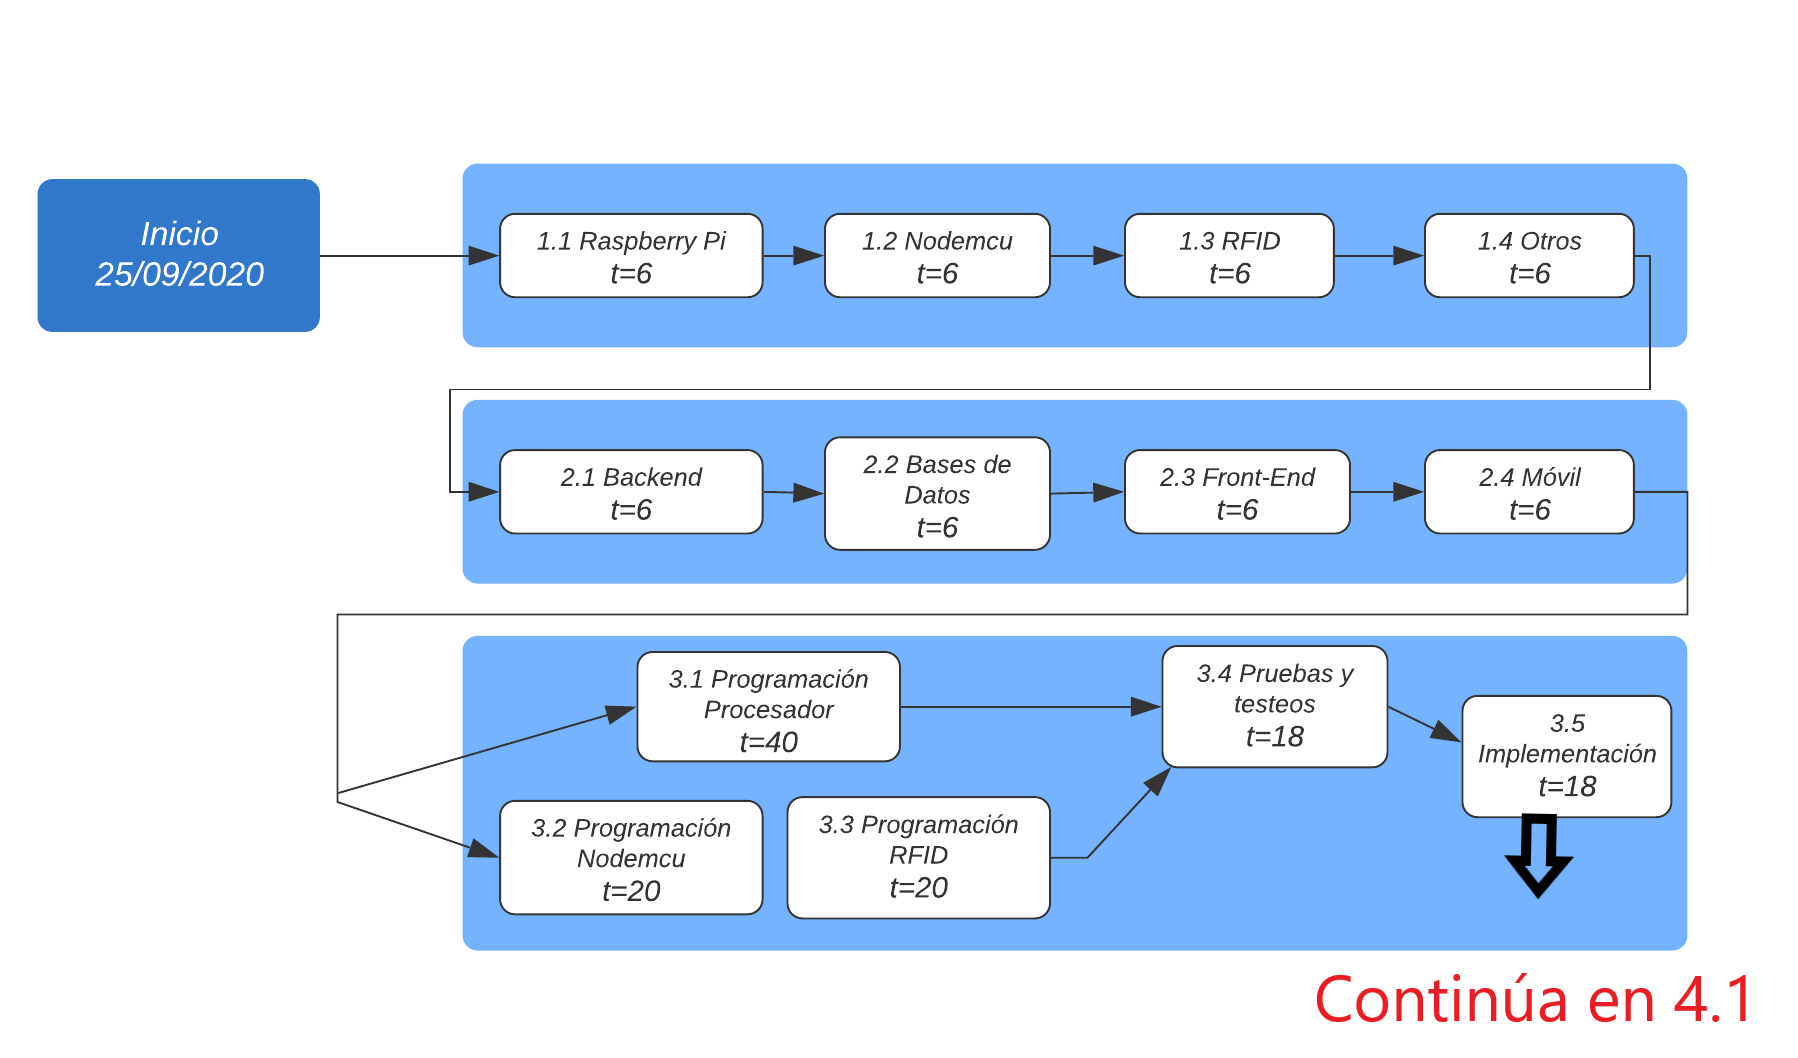
\includegraphics[width=.9\textwidth]{./Figuras/AON-1.png}
\caption{Diagrama en \textit{Activity on Node}}
\label{fig:AoN}
\end{figure}
\begin{figure}[htpb]
\centering 
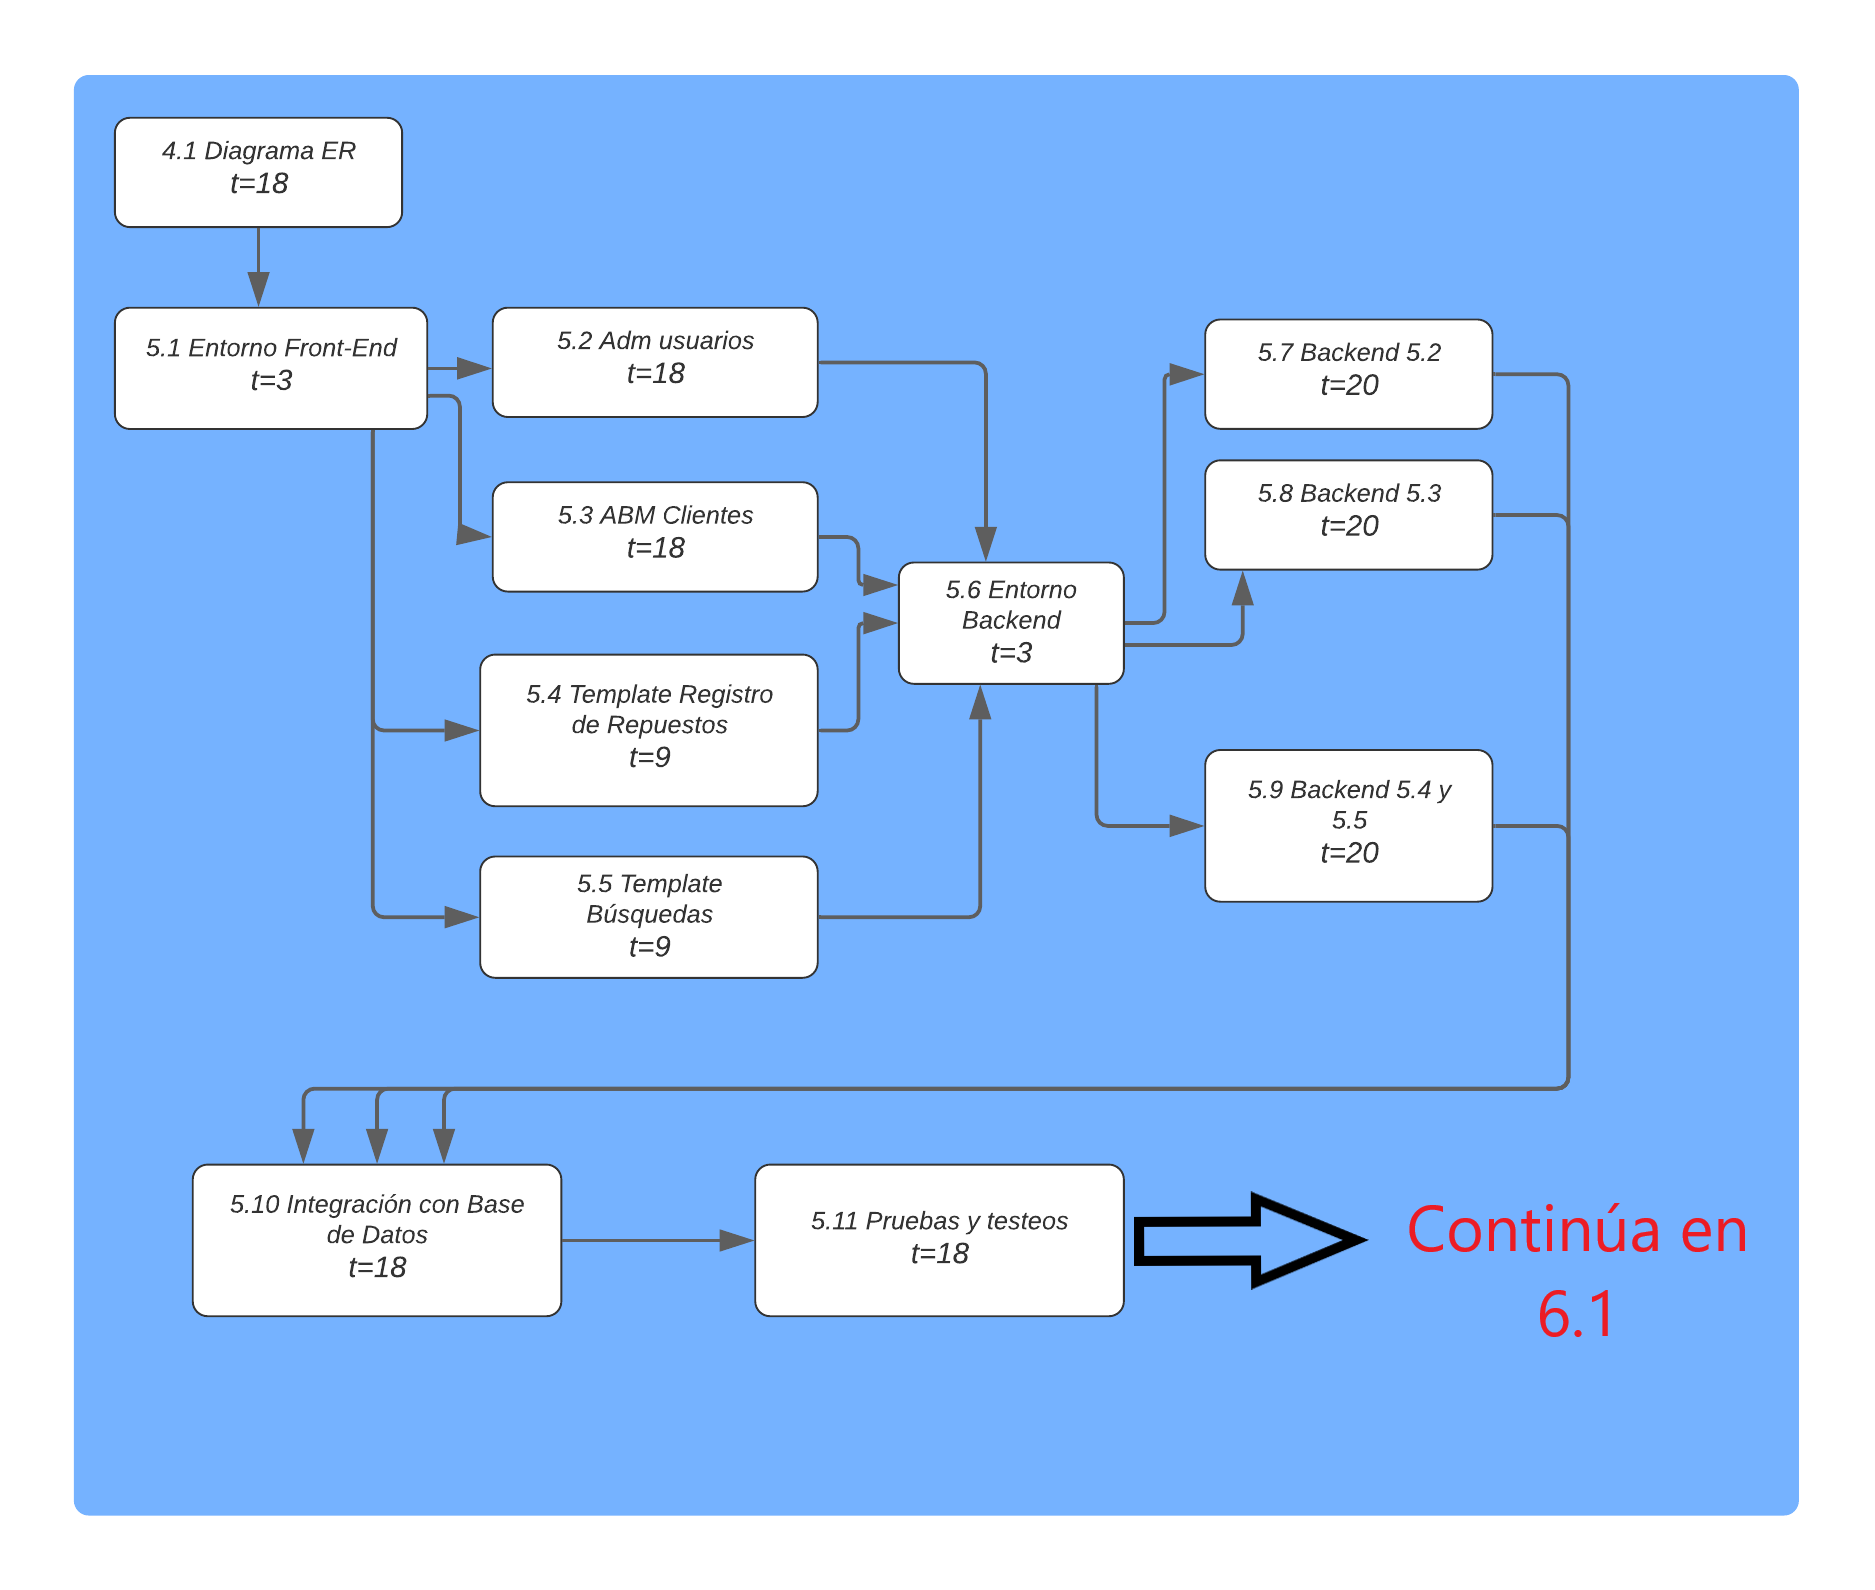
\includegraphics[width=.9\textwidth]{./Figuras/AON-2.png}
\caption{Diagrama en \textit{Activity on Node}}
\label{fig:AoN}
\end{figure}

\begin{figure}[htpb]
\centering 
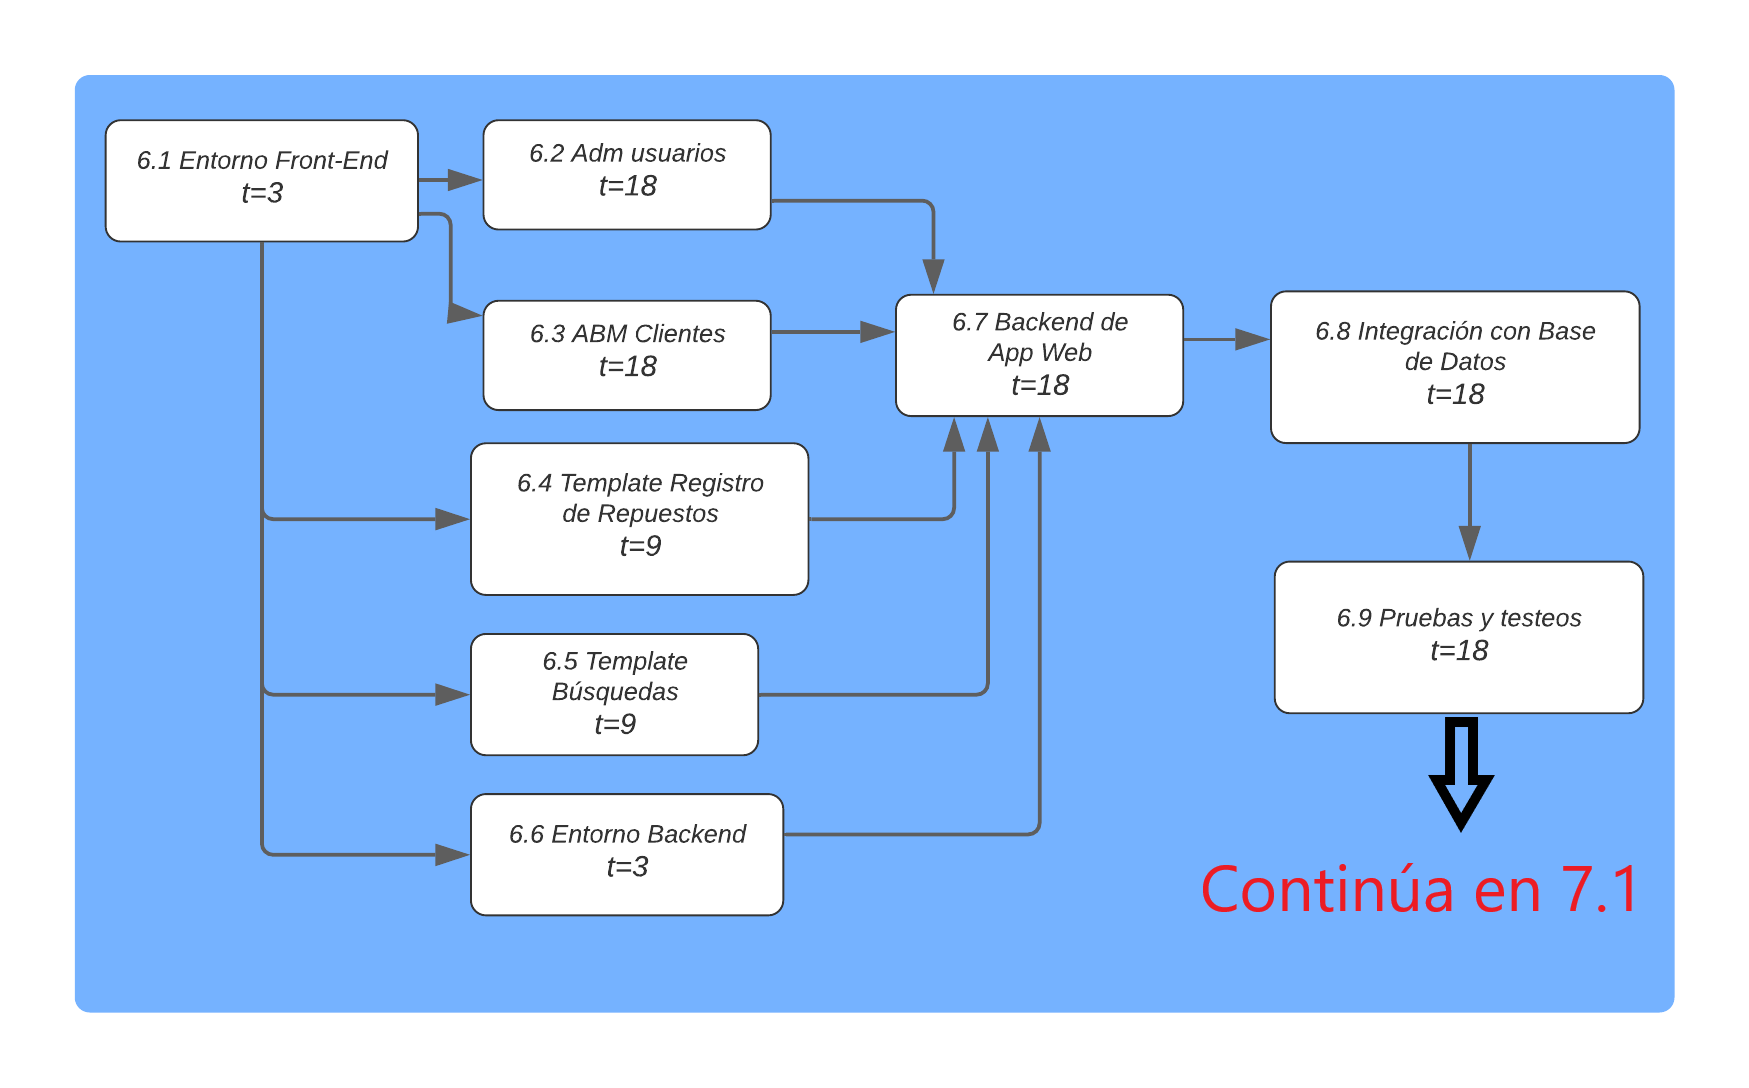
\includegraphics[width=.9\textwidth]{./Figuras/AON-3.png}
\caption{Diagrama en \textit{Activity on Node}}
\label{fig:AoN}
\end{figure}

\begin{figure}[htpb]
\centering 
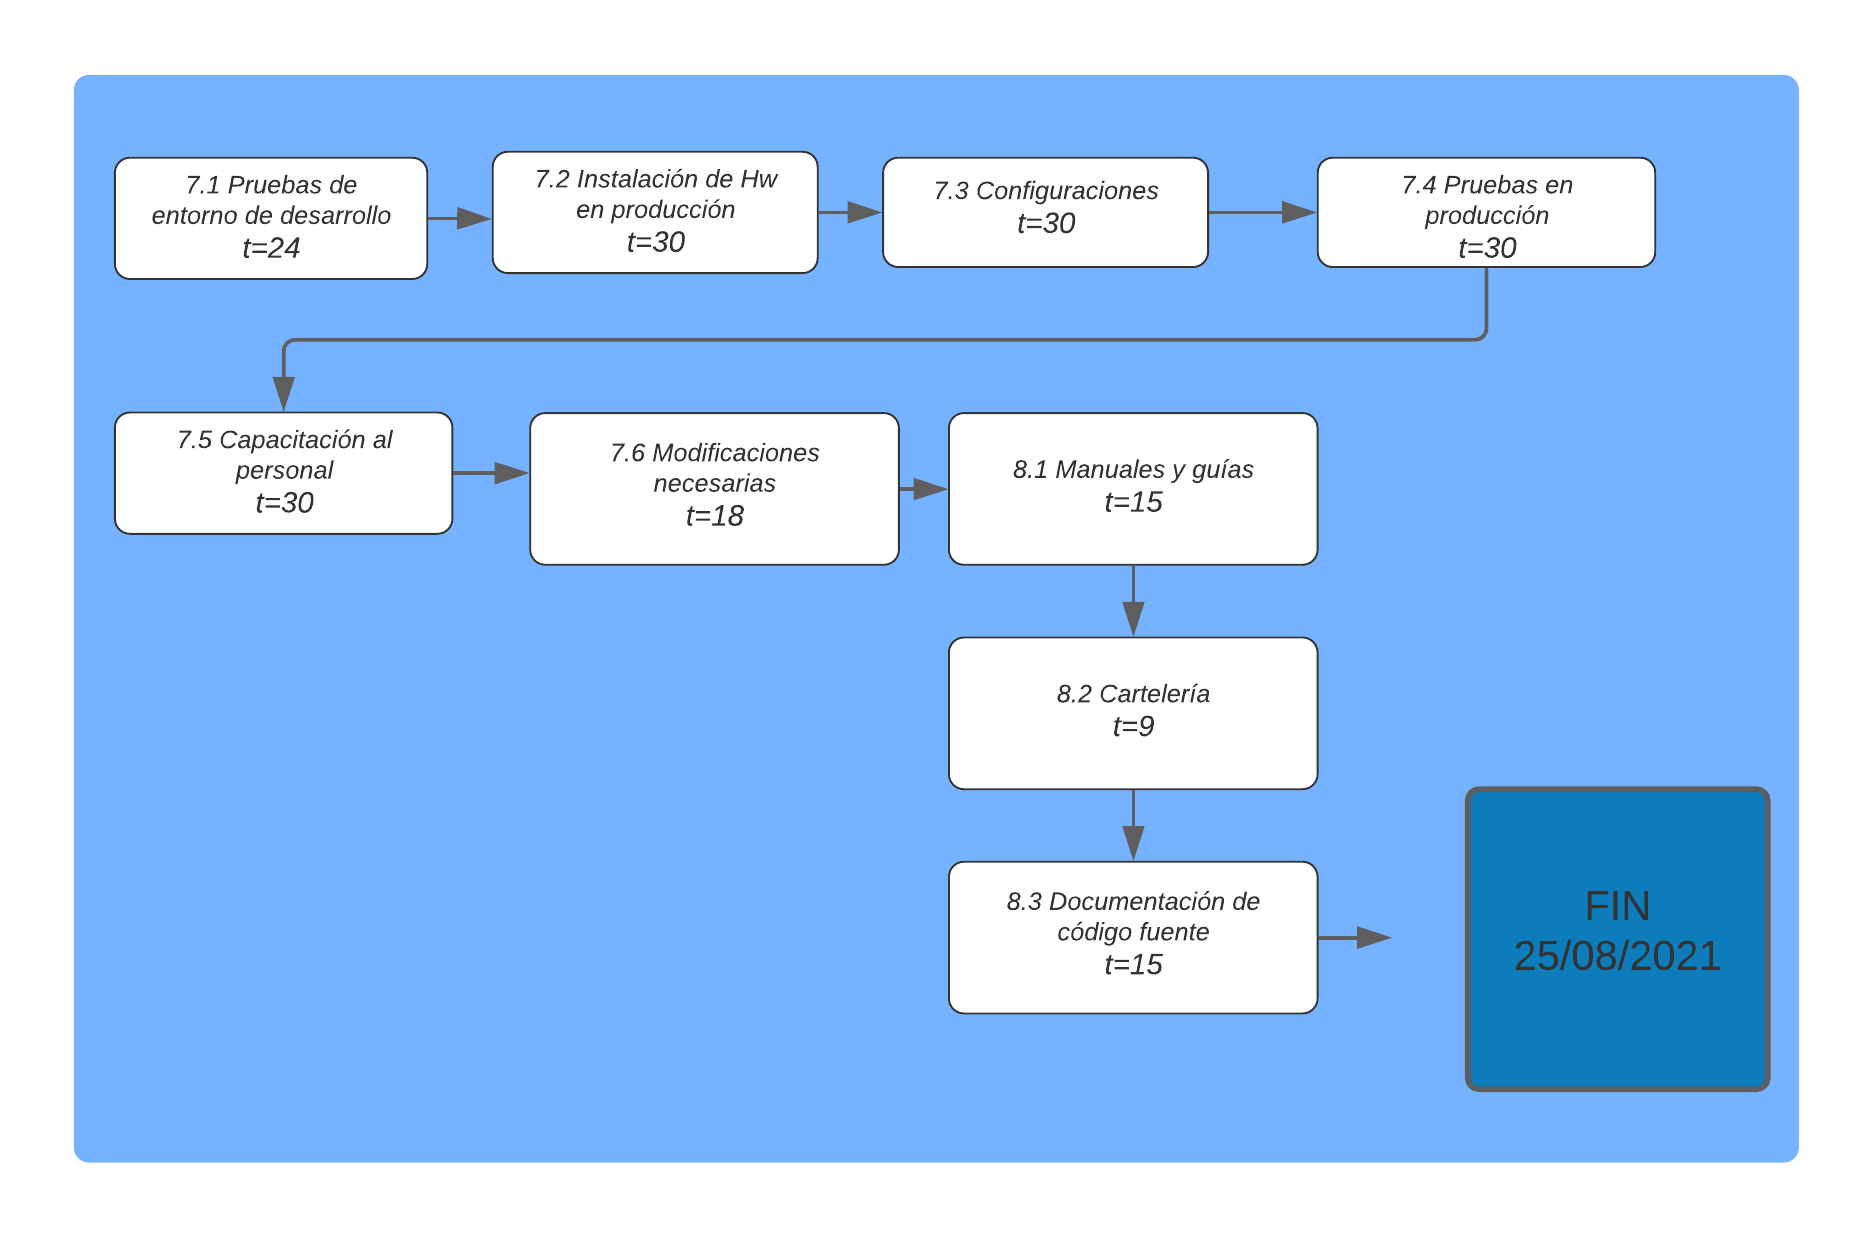
\includegraphics[width=.9\textwidth]{./Figuras/AON-4.png}
\caption{Diagrama en \textit{Activity on Node}}
\label{fig:AoN}
\end{figure}

Unidad de tiempo expresada en horas.
\\Camino crítico: tareas: 1.1 - 1.2 - 1.3 - 1.4 - 2.1 - 2.2 - 2.3 - 2.4 - 3.1 - 3.4 - 3.5 - 4.1 - 5.1 - 5.2 - 5.6 - 5.7 - 5.10 - 5.11 - 6.1 - 6.2 - 6.7 - 6.8 - 6.9 - 7.1 - 7.2 - 7.3 - 7.4 - 7.5 - 7.6 - 8.1 .
\\Cantidad de horas del camino crítico: 474 horas.


\section{8. Diagrama de Gantt}
\label{sec:gantt}

\begin{consigna}{black}
%Utilizar el software Gantter for Google Drive o alguno similar para dibujar el diagrama de Gantt.

%Existen muchos programas y recursos \textit{online} para hacer diagramas de gantt, entre las cuales destacamos:

%\begin{itemize}
%\item Planner
%\item GanttProject
%\item Trello + \textit{plugins}. En el siguiente link hay un tutorial oficial: \\ \url{https://blog.trello.com/es/diagrama-de-gantt-de-un-proyecto}
%\item Creately, herramienta online colaborativa. \\\url{https://creately.com/diagram/example/ieb3p3ml/LaTeX}
%\item Se puede hacer en latex con el paquete \textit{pgfgantt}\\ \url{http://ctan.dcc.uchile.cl/graphics/pgf/contrib/pgfgantt/pgfgantt.pdf}
%\end{itemize}

%Pegar acá una captura de pantalla del diagrama de Gantt, cuidando que la letra sea suficientemente grande como para ser legible. 
%Si el diagrama queda demasiado ancho, se puede pegar primero la ``tabla'' del Gantt y luego pegar la parte del diagrama de barras del diagrama de Gantt.

%Configurar el software para que en la parte de la tabla muestre los códigos del EDT (WBS).\\
%Configurar el software para que al lado de cada barra muestre el nombre de cada tarea.\\
%Revisar que la fecha de finalización coincida con lo indicado en el Acta Constitutiva.

%En la figura \ref{fig:gantt}, se muestra un ejemplo de diagrama de gantt realizado con el paquete de \textit{pgfgantt}. En la plantilla pueden ver el código que lo genera y usarlo de base para construir el propio.

%\begin{figure}[htbp]
%\begin{center}
%\begin{ganttchart}{1}{12}
%  \gantttitle{2020}{12} \\
%  \gantttitlelist{1,...,12}{1} \\
%  \ganttgroup{Group 1}{1}{7} \\
%  \ganttbar{Task 1}{1}{2} \\
%  \ganttlinkedbar{Task 2}{3}{7} \ganttnewline
%  \ganttmilestone{Milestone o hito}{7} \ganttnewline
%  \ganttbar{Final Task}{8}{12}
%  \ganttlink{elem2}{elem3}
%  \ganttlink{elem3}{elem4}
%\end{ganttchart}
%\end{center}
%\caption{Diagrama de gantt de ejemplo}
%\label{fig:gantt}
%\end{figure}

\begin{figure}[htpb]
\centering 
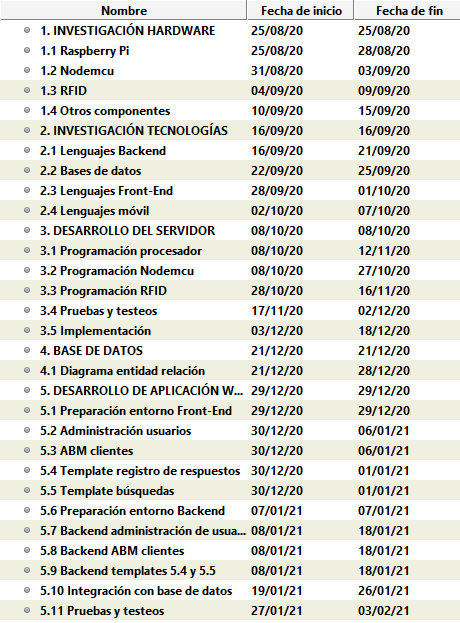
\includegraphics[width=.8\textwidth]{./Figuras/Gantt-2-1.png}
\caption{Diagrama de \textit{Gantt}. Tabla de tareas}
\label{fig:AoN}
\end{figure}
\begin{figure}[htpb]
\centering 
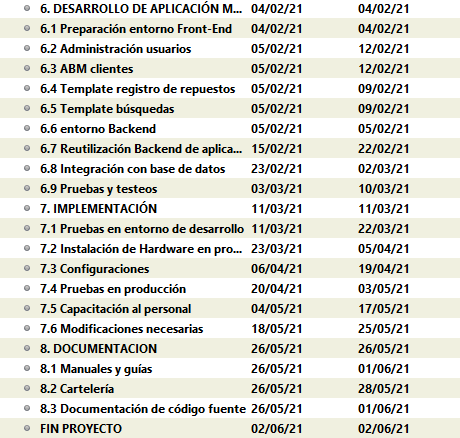
\includegraphics[width=.8\textwidth]{./Figuras/Gantt-2-2.png}
\caption{Diagrama de \textit{Gantt}. Tabla de tareas}
\label{fig:AoN}
\end{figure}

\begin{figure}[htpb]
\centering 
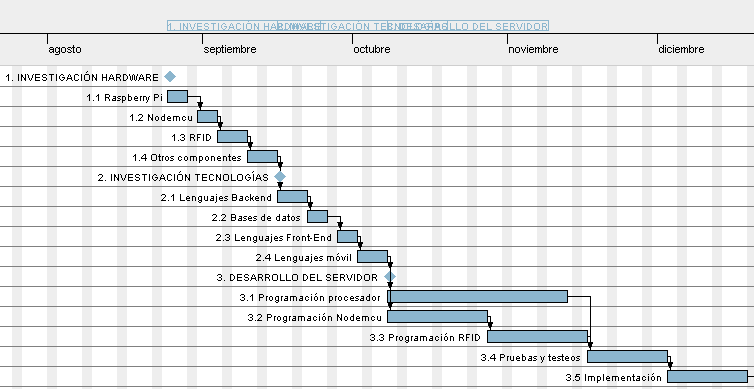
\includegraphics[width=.9\textwidth]{./Figuras/Gantt-3-1.png}
\caption{Diagrama de \textit{Gantt}}
\label{fig:AoN}
\end{figure}
\begin{figure}[htpb]
\centering 
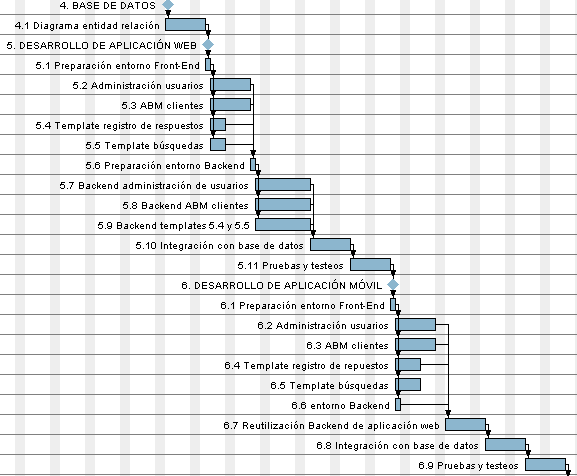
\includegraphics[width=.9\textwidth]{./Figuras/Gantt-3-2.png}
\caption{Diagrama de \textit{Gantt}}
\label{fig:AoN}
\end{figure}
\begin{figure}[htpb]
\centering 
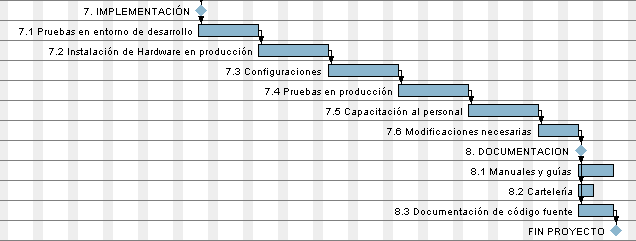
\includegraphics[width=.9\textwidth]{./Figuras/Gantt-3-3.png}
\caption{Diagrama de \textit{Gantt}}
\label{fig:AoN}
\end{figure}



\end{consigna}

\section{9. Matriz de uso de recursos de materiales}
\label{sec:recursos}


\begin{table}[htpb]
\label{tab:recursos}
\centering
\begin{tabularx}{\linewidth}{@{}|c|X|X|X|X|c|@{}}
\hline
\cellcolor[HTML]{C0C0C0} & \cellcolor[HTML]{C0C0C0} & \multicolumn{4}{c|}{\cellcolor[HTML]{C0C0C0}Recursos requeridos (horas)} \\ \cline{3-6} 
\multirow{-2}{*}{\cellcolor[HTML]{C0C0C0}\begin{tabular}[c]{@{}c@{}}Código\\ WBS\end{tabular}} & \multirow{-2}{*}{\cellcolor[HTML]{C0C0C0}\begin{tabular}[c]{@{}c@{}}Nombre \\ tarea\end{tabular}} & Raspberry Pi & Nodemcu & RFID & PC \\ \hline
1.1 &Investigación Raspberry Pi 	 &3  &  &  &3  \\ \hline
1.2 &Investigación Nodemcu  		&1  &3  &  &3  \\ \hline
1.3 &Investigación RFID		 	 	&1 &1  &3  &3  \\ \hline
1.4 &Otros componentes  &  &  &  &6  \\ \hline
2. &Investigación sobre tecnologías  &  &  &  &24  \\ \hline
3.1 &Programación procesador  &10  &  &  &40  \\ \hline
3.2 &Programación Nodemcu  &  &10  &  &20  \\ \hline
3.3 &Programación RFID  &5  &5  &10  &20  \\ \hline
3.4 &Pruebas y testeos  &9  &6  &3  &18  \\ \hline
3.5 &Implementación  &9  &6  &3  &18  \\ \hline
4.1 &Diagrama entidad relación  &  &  &  &18  \\ \hline
5 &Desarrollo de aplicación web  &  &  &  &156  \\ \hline
6 &Desarrollo de aplicación móvil  &  &  &  &114  \\ \hline
7.1 &Pruebas en entorno de desarrollo  &6  &6  &6  &24  \\ \hline
7.2 &Instalación de hardware en producción  &12  &12  &6  &  \\ \hline
7.3 &Configuraciones  &10  &10  &10  &20  \\ \hline
7.4 &Pruebas en producción   &9  &6  &3  &22  \\ \hline 
7.5 &Capacitación de personal  &6  &3  &1  &20  \\ \hline
8 &Documentación  &  &  &  &39  \\ \hline


\end{tabularx}%
\end{table}


\section{10. Presupuesto detallado del proyecto}
\label{sec:presupuesto}

\begin{consigna}{black}
%Si el proyecto es complejo entonces separarlo en partes:
%\begin{itemize}
%\item Un total global, indicando el subtotal acumulado por cada una de las áreas.
%\item El desglose detallado del subtotal de cada una de las áreas.
%\end{itemize}

%IMPORTANTE: No olvidarse de considerar los COSTOS INDIRECTOS.

\end{consigna}

\begin{table}[htpb]
\centering
\begin{tabularx}{\linewidth}{@{}|X|c|r|r|@{}}
\hline
\rowcolor[HTML]{C0C0C0} 
\multicolumn{4}{|c|}{\cellcolor[HTML]{C0C0C0}COSTOS DIRECTOS} \\ \hline
\rowcolor[HTML]{C0C0C0} 
Descripción &
  \multicolumn{1}{c|}{\cellcolor[HTML]{C0C0C0}Cantidad} &
  \multicolumn{1}{c|}{\cellcolor[HTML]{C0C0C0}Valor unitario} &
  \multicolumn{1}{c|}{\cellcolor[HTML]{C0C0C0}Valor total} \\ \hline
 Horas de Ingeniería &   \multicolumn{1}{c|}{653} &  \multicolumn{1}{c|}{800} & \multicolumn{1}{c|}{522400} \\ \hline
Raspberry Pi&  \multicolumn{1}{c|}{1} &  \multicolumn{1}{c|}{15000} &  \multicolumn{1}{c|}{15000} \\ \hline
Nodemcu&  \multicolumn{1}{c|}{4} &  \multicolumn{1}{c|}{900} &  \multicolumn{1}{c|}{3600} \\ \hline
RFID &  \multicolumn{1}{c|}{50} &  \multicolumn{1}{c|}{40} &  \multicolumn{1}{c|}{2000} \\ \hline
Cables y otros electricidad &  \multicolumn{1}{c|}{1} &  \multicolumn{1}{c|}{3000} &  \multicolumn{1}{c|}{3000} \\ \hline
Cajas plásticas&  \multicolumn{1}{c|}{40} &  \multicolumn{1}{c|}{100} &  \multicolumn{1}{c|}{4000} \\ \hline

\multicolumn{3}{|c|}{SUBTOTAL} &
  \multicolumn{1}{c|}{550000} \\ \hline
\rowcolor[HTML]{C0C0C0} 
\multicolumn{4}{|c|}{\cellcolor[HTML]{C0C0C0}COSTOS INDIRECTOS} \\ \hline
\rowcolor[HTML]{C0C0C0} 
Descripción &
  \multicolumn{1}{c|}{\cellcolor[HTML]{C0C0C0}Cantidad} &
  \multicolumn{1}{c|}{\cellcolor[HTML]{C0C0C0}Valor unitario} &
  \multicolumn{1}{c|}{\cellcolor[HTML]{C0C0C0}Valor total} \\ \hline
\multicolumn{1}{|l|}{25\% de los costos directos	} &1    &137500    &137500    \\ \hline
	\multicolumn{1}{|l|}{} &    &    &    \\ \hline
	\multicolumn{1}{|l|}{} &    &    &    \\ \hline
	\multicolumn{3}{|c|}{SUBTOTAL} &
  \multicolumn{1}{c|}{137500} \\ \hline
\rowcolor[HTML]{C0C0C0}
\multicolumn{3}{|c|}{TOTAL} &687500
   \\ \hline
\end{tabularx}%
\end{table}


\section{11. Matriz de asignación de responsabilidades}
\label{sec:responsabilidades}
\begin{consigna}{black}
%Establecer la matriz de asignación de responsabilidades y el manejo de la autoridad completando la siguiente tabla:

\begin{table}[htpb]
\centering
\resizebox{\textwidth}{!}{%
\begin{tabular}{|c|c|c|c|c|c|}
\hline
\rowcolor[HTML]{C0C0C0} 
\cellcolor[HTML]{C0C0C0} &
  \cellcolor[HTML]{C0C0C0} &
  \multicolumn{4}{c|}{\cellcolor[HTML]{C0C0C0}Listar todos los nombres y roles del proyecto} \\ \cline{3-6} 
\rowcolor[HTML]{C0C0C0} 
\cellcolor[HTML]{C0C0C0} &
  \cellcolor[HTML]{C0C0C0} &
  Responsable &
  Orientador &
  Codirector &
  Cliente \\ \cline{3-6} 
\rowcolor[HTML]{C0C0C0} 
\multirow{-3}{*}{\cellcolor[HTML]{C0C0C0}\begin{tabular}[c]{@{}c@{}}Código\\ WBS\end{tabular}} &
  \multirow{-3}{*}{\cellcolor[HTML]{C0C0C0}Nombre de la tarea} &
  \authorname &
  \supname &
  Miguel del Valle &
  \clientename \\ \hline
 1 & Investigación hardware & P & A & C &  \\ \hline
 2 & Investigación sobre tecnologías & P  & A & C &  \\ \hline
 3 & Desarrollo de servidor & P & A & C & I \\ \hline
 4 & Desarrollo de base de datos & P & I & I &  \\ \hline
 5 & Desarrollo de aplicación web & P & A & C & I  \\ \hline
 6 & Desarrollo de aplicación móvil & P & A & C & I  \\ \hline
 7 & Implementación & P & A & C & A  \\ \hline
 8 & Documentación & P & A & C & I  \\ \hline
\end{tabular}%
}
\end{table}

{\footnotesize
Referencias:
\begin{itemize}
	\item P = Responsabilidad Primaria
	\item S = Responsabilidad Secundaria
	\item A = Aprobación
	\item I = Informado
	\item C = Consultado
\end{itemize}
} %footnotesize

%Una de las columnas debe ser para el Director, ya que se supone que participará en el proyecto.
%A su vez se debe cuidar que no queden muchas tareas seguidas sin ``A'' o ``I''.

%Importante: es redundante poner ``I/A'' o ``I/C'', porque para aprobarlo o responder consultas primero la persona debe ser informada.

\end{consigna}

\section{12. Gestión de riesgos}
\label{sec:riesgos}

\begin{consigna}{black}
a) Identificación de los riesgos y estimación de sus consecuencias:
 
\begin{itemize}
\item Severidad (S): mientras más severo, más alto es el número. Rango: 0 a 10\\
\item Probabilidad de ocurrencia (O): mientras más probable, más alto es el número. Rango: 0 a 10\\
\end{itemize}   

Riesgo 1: bajo rendimiento del hardware seleccionado para el servidor.
\begin{itemize}
\item Severidad (10): implicaría el retraso en los procesos de la organización, causando pérdidas económicas y generando un mal servicio a los clientes.
\item Ocurrencia (4): se ha investigado el hardware en cuestión y comparado su rendimiento con los requerimientos del sistema. El resultado fue favorable al rendimiento.
\end{itemize}

Riesgo 2: no cumplir con la fecha de entrega.
\begin{itemize}
\item Severidad (8): implica retrasar la aprobación de la especialización y no cumplir con lo esperado por el cliente.
\item Ocurrencia (3): dados los estudios realizados en este plan, se estima que existen escasas probabilidades de no cumplir con la fecha pactada. 
\end{itemize}

Riesgo 3: fallas en la transmisión de datos entre componentes.
\begin{itemize}
\item Severidad (9): implicaría el mal funcionamiento de todo el sistema y la entrega de datos imprecisos a los usuarios y los clientes de la empresa.
\item Ocurrencia (7): se estima que al utilizar comunicaciones inalámbricas pueden existir interferencias entre componentes.
\end{itemize}

Riesgo 4: desinterés por parte del personal en la utilización de los servicios.
\begin{itemize}
\item Severidad (10): implicaría el fracaso de este producto y una pérdida de inversión monetaria y de tiempo.
\item Ocurrencia (2): en las entrevistas realizadas el personal se mostró muy interesado en el producto ya que conlleva una manera de trabajar más rápida y cómoda para todos ellos.
\end{itemize}

Riesgo 5: incremento del costo de los componentes necesarios para el proyecto.
\begin{itemize}
\item Severidad (5): conlleva el aumento del presupuesto total para el cliente.
\item Ocurrencia (10): los productos están en constante aumento por lo que es importante adquirirlos con anticipación.
\end{itemize}


b) Tabla de gestión de riesgos:      (El RPN se calcula como RPN=SxO)
\begin{table}[htpb]
\centering
\begin{tabularx}{\linewidth}{@{}|X|c|c|c|c|c|c|@{}}
\hline
\rowcolor[HTML]{C0C0C0} 
Riesgo & S & O & RPN & S* & O* & RPN* \\ \hline
 Riesgo 1: bajo rendimiento del hardware seleccionado para el servidor. &10   &4   &40     &6    &2    &12      \\ \hline
 Riesgo 2: no cumplir con la fecha de entrega.  &8   &3   &24     &-    & -   & -     \\ \hline
 Riesgo 3: fallas en la transmisión de datos entre componentes. &9   &7   & 63    &6    &5    &30      \\ \hline
  Riesgo 4: desinterés por parte del personal en la utilización de los servicios.&10   &2   &20     &-    &  -  & -     \\ \hline
   Riesgo 5: incremento del costo de los componentes necesarios para el proyecto. &5   &10   &50     &2    &6    &12      \\ \hline
\end{tabularx}
\end{table}

\end{consigna}
\begin{consigna}{black}
\begin{itemize}

\item Criterio adoptado: 
se tomarán medidas de mitigación en los riesgos cuyos números de RPN sean mayores a 40.

\item Nota: los valores marcados con (*) en la tabla corresponden luego de haber aplicado la mitigación.

\end{itemize}
c) Plan de mitigación de los riesgos que originalmente excedían el RPN máximo establecido:
 

Riesgo 1: bajo rendimiento del hardware seleccionado para el servidor.

- Severidad (6): debido a que el sistema consta de varios módulos, se podrán implementar algunos servicios por fuera de la placa raspberry, como ser la base de datos o el servidor web. Estos servicios pueden estar alojados en una de las PC de la organización o inclusive en la nube. De esta manera se minimizan los requerimientos de procesamiento a este componente.

- Probabilidad de ocurrencia (2): si se migran servicios de este componente disminuiría considerablemente la demanda de procesamiento.

Riesgo 3: fallas en la transmisión de datos entre componentes.
 \\- Severidad (6): se implementará un lector adicional y la posibilidad de la entrada manual de datos en una interfaz para casos de contingencia.
 \\- Probabilidad de ocurrencia (5): al tener canales alternativos se minimizan las posibilidades de quedarse sin comunicación con el servidor.
 
Riesgo 5: incremento del costo de los componentes necesarios para el proyecto.
\\- Severidad (2): la mayoría de los componentes ya fueron adquiridos, para el resto de componentes se notificará inmediatamente al cliente la recomendación de realizar la compra.
 \\- Probabilidad de ocurrencia (6): una vez que se adquieran todos los componentes no influiría el aumento en el mercado de los mismos ya que restaría sólo la compra de accesorios mínimos.

\end{consigna}


\section{13. Gestión de la calidad}
\label{sec:calidad}

\begin{consigna}{black}

\begin{enumerate}
\item Grupo de requerimientos asociados con el Servidor:
	\begin{enumerate}
	\item Comunicación websocket con Esp32 (lectores RFID)
	\begin{itemize}
	\item Verificación: pruebas de transmisión de datos entre Esp32 y Raspberry a través de wifi.  
	\item Validación: constatar con el cliente que al pasar una tarjeta por el lector RFID se actualizan los datos en el servidor.  
	\end{itemize}
	\item Almacenamiento de base de datos (MySql,MariaDB o PostgreSql)
	\begin{itemize}
	\item Verificación: comprobación de almacenamiento de datos en gestor de base de datos correspondiente.
	\item Validación: muestra de datos en gestor de base de datos instalado en producción, actualización de datos en tiempo real y muestra de los mismos.  
	\end{itemize}
	\item Procesamiento en lenguaje de nivel medio (Python)
	\begin{itemize}
	\item Verificación: se utilizará este lenguaje para programar el procesador. 
	\item Validación: se informará la versión del lenguaje utilizado al cliente en la documentación.  
	\end{itemize}
	\item Tecnologías Rest para comunicación con los demás servicios.
	\begin{itemize}
	\item Verificación: pruebas en transmisión de datos por medio de http rest. 
	\item Validación: pruebas reales en entorno de producción a modo de corroborar la actualización inmediata de datos.  
	\end{itemize}
	\end{enumerate}
\item Grupo de requerimientos asociados con Aplicación Web
	\begin{enumerate}
	\item Registro de repuestos entrantes
	\begin{itemize}
	\item Verificación: simular entrada de registros por medio de todos los canales implicados. 
	\item Validación: realizar registros reales en entorno de producción.  
	\end{itemize}
	\item Actualización inmediata de estados de procesos
	\begin{itemize}
	\item Verificación: análisis de demora en actualización de datos al realizar un registro nuevo. 
	\item Validación: constatar la actualización inmediata de los datos en las interfaces correspondientes.  
	\end{itemize}
	\item ABM de clientes
	\begin{itemize}
	\item Verificación: ingreso de registros simulados para corroborar el funcionamiento de este módulo. 
	\item Validación: ingresar de registros reales en entorno de producción y constatar su almacenamiento.
	\end{itemize}
	\item Búsqueda avanzada: por fecha, por cliente, por estado (para usuarios y administradores)
	\begin{itemize}
	\item Verificación: pruebas con distintos roles en las aplicaciones, ingresando datos de búsqueda. 
	\item Validación: corroborar en entorno de producción con datos reales.  
	\end{itemize}
	\item Búsqueda de repuestos por id (para clientes) sin necesidad de acceso con usuario y contraseña.
	\begin{itemize}
	\item Verificación: corroborar las búsquedas desde navegadores en modo privado a fin de que no intervengan sesiones previas ni cookies.  
	\item Validación: realizar pruebas con repuestos ingresados y verificar en cada cambio de estado.  
	\end{itemize}
	\item Roles: Usuario, Administrador, Cliente. Con nombre de usuario y contraseña excepto clientes.
	\begin{itemize}
	\item Verificación: pruebas de navegación con usuarios simulados de cada rol por todas las interfaces. Pruebas de acceso mediante url a secciones no autorizadas para ese rol. 
	\item Validación: pruebas similares con los usuarios reales de la empresa.  
	\end{itemize}
	\item Diseño web adaptable (responsive design) y amigable.
	\begin{itemize}
	\item Verificación: acceso desde distintos dispositivos al sistema web. Pruebas con herramientas para simular diferentes pantallas.
	\item Validación: acceso desde dispositivos varios en la empresa.  
	\end{itemize}
	\end{enumerate}
\item Grupo de requerimientos asociados con Aplicación Móvil
	\begin{enumerate}
	\item Actualización inmediata de estados de procesos
	\begin{itemize}
	\item Verificación: acceso desde la aplicación web y verificación en cambios de proceso. Análisis del tiempo de demora.
	\item Validación: corroborar el cambio de estado de procesos en aplicación móvil.  
	\end{itemize}
	\item Búsqueda avanzada: por fecha, por cliente, por estado (para usuarios y administradores)
	\begin{itemize}
	\item Verificación: pruebas con distintos usuarios en la aplicación, ingresando datos de búsqueda. 
	\item Validación: corroborar en entorno de producción con datos reales desde distintos dispositivos.  
	\end{itemize}
	\item Búsqueda de repuestos por id (para clientes) sin necesidad de acceso con usuario y contraseña.
	\begin{itemize}
	\item Verificación: corroborar las búsquedas desde la aplicación ingresando con diferentes usuarios y desde varios dispositivos en simultáneo (al menos dos).  
	\item Validación: realizar pruebas con repuestos ingresados y verificar en cada cambio de estado.  
	\end{itemize}
	\item Roles: Usuario, Administrador, Cliente. Con nombre de usuario y contraseña excepto clientes.
	\begin{itemize}
	\item Verificación: pruebas de acceso con usuarios simulados de cada rol por todas las secciones de la aplicación. 
	\item Validación: pruebas similares con los usuarios reales de la empresa.  
	\end{itemize}
	\item Diseño amigable.
	\begin{itemize}
	\item Verificación: realizar pruebas con usuarios nuevos sin previa lectura de documentación. 
	\item Validación: corroborar que la navegación por la aplicación sea intuitiva con usuarios nuevos.  
	\end{itemize}
	\end{enumerate}
\end{enumerate}

\end{consigna}

\section{14. Comunicación del proyecto}
\label{sec:comunicaciones}

El plan de comunicación del proyecto es el siguiente:

\begin{table}[htpb]
\centering
\begin{tabularx}{\linewidth}{@{}|X|C{2.4cm}|C{3cm}|C{1.8cm}|C{2cm}|C{2.1cm}|@{}}
\hline
\rowcolor[HTML]{C0C0C0} 
\multicolumn{6}{|c|}{\cellcolor[HTML]{C0C0C0}PLAN DE COMUNICACIÓN DEL PROYECTO}           \\ \hline
\rowcolor[HTML]{C0C0C0} 
¿Qué comunicar? & Audiencia & Propósito & Frecuencia & Método de comunicac. & Responsable \\ \hline
 Desarrollo del servidor & Director y codirector&Informar avance&Cada 15 días&Email & Pablo Arancibia            \\ \hline
Desarrollo de base de datos & Director y codirector&Corroborar buen diseño&Al finalizar la base de datos&Email &Pablo Arancibia \\ \hline
Desarrollo de aplicación web & Director y codirector&Informar avances y corroborar buen diseño y funcionalidad &Cada 15 días &Email &Pablo Arancibia             \\ \hline
Desarrollo de aplicación móvil & Director y codirector&Informar avances y corroborar buen diseño y funcionalidad &Cada 15 días &Email &Pablo Arancibia\\ \hline
Implemen- tación & Director, codirector y cliente&Informar avances y buena implementación&Semanalmente&Email y presencial con el cliente  &Pablo Arancibia \\ \hline
Documen- tación & Director, codirector y cliente &Informar finalización y entrega&Al finalizar la documentación&Email &Pablo Arancibia             \\ \hline
Finalización del proyecto & Director, codirector, cliente  e interesados&Informar finalización del proyecto &Al finalizar el proyecto     &Email y presencial con el cliente e interesados  & Pablo Arancibia            \\ \hline
\end{tabularx}
\end{table}

\section{15. Gestión de compras}
\label{sec:compras}

\begin{consigna}{black}
Todos los componentes detallados en el presupuesto de este documento pueden ser adquiridos por https://www.mercadolibre.com.ar 
\end{consigna}

\section{16. Seguimiento y control}
\label{sec:seguimiento}
\begin{consigna}{black}
\begin{longtable}{|m{1cm}|m{3.5cm}|m{2.2cm}|m{2cm}|m{3cm}|m{1.5cm}|}
\hline
\rowcolor[HTML]{C0C0C0} 
\multicolumn{6}{|c|}{\cellcolor[HTML]{C0C0C0}SEGUIMIENTO DE AVANCE}                                                                       \\ \hline
\rowcolor[HTML]{C0C0C0} 
Tarea del WBS 			& Indicador de avance & Frecuencia de reporte & Resp. de seguimiento & Persona a ser informada & Método de comunic. \\ \hline
\endfirsthead

\hline
\rowcolor[HTML]{C0C0C0} 
\multicolumn{6}{c}{\cellcolor[HTML]{C0C0C0}SEGUIMIENTO DE AVANCE}                                                                       \\ \hline
\rowcolor[HTML]{C0C0C0} 
Tarea del WBS 			& Indicador de avance & Frecuencia de reporte & Resp. de seguimiento & Persona a ser informada & Método de comunic. \\ \hline
\endhead

\multicolumn{6}{c}{Continúa}
\endfoot

\endlastfoot

1.1	& Información final obtenida  & Única vez al finalizar & \authorname & \supname y \cosupname & email \\ \hline
1.2	&Información final obtenida  & Única vez al finalizar & \authorname & \supname y \cosupname & email \\ \hline
1.3	& Información final obtenida  & Única vez al finalizar & \authorname & \supname y \cosupname & email \\ \hline
1.4	&Información final obtenida  & Única vez al finalizar & \authorname & \supname y \cosupname & email \\ \hline
2.1	& Información final obtenida  & Única vez al finalizar & \authorname & \supname y \cosupname & email \\ \hline
2.2	& Información final obtenida & Única vez al finalizar & \authorname & \supname y \cosupname & email \\ \hline
2.3	& Información final obtenida  & Única vez al finalizar & \authorname & \supname y \cosupname & email \\ \hline
2.4	& Información final obtenida  & Única vez al finalizar & \authorname & \supname y \cosupname & email \\ \hline
3.1	& Cada módulo nuevo realizado  & Semanal & \authorname & \supname y \cosupname & email \\ \hline
3.2	& Cada función nueva realizada  & Semanal & \authorname & \supname y \cosupname & email \\ \hline
3.3	& Cada función nueva realizada  & Semanal & \authorname & \supname y \cosupname & email \\ \hline
3.4	& Cantidad de pruebas realizadas y sus resultados  & Semanal & \authorname & \supname y \cosupname & email \\ \hline
3.5	& Implementación con cada componente  & Semanal & \authorname & \supname y \cosupname & email \\ \hline
4.1	& Cantidad de tablas y sus relaciones diseñadas  & Única vez al finalizar & \authorname & \supname y \cosupname & email \\ \hline
5.1	& Software instalado y en funcionamiento &Única vez al finalizar& \authorname & \supname y \cosupname & email \\ \hline
5.2	& Cada interfaz realizada &Semanal& \authorname & \supname y \cosupname & email \\ \hline
5.3	& Cada interfaz realizada &Semanal& \authorname & \supname y \cosupname & email \\ \hline
5.4	& Cada interfaz realizada &Semanal& \authorname & \supname y \cosupname & email \\ \hline
5.5	& Cada interfaz realizada &Semanal& \authorname & \supname y \cosupname & email \\ \hline
5.6	& Software instalado y en funcionamiento&Única vez al finalizar& \authorname & \supname y \cosupname & email \\ \hline
5.7	& Cada funcionalidad finalizada sobre cada interfaz &Semanal& \authorname & \supname y \cosupname & email \\ \hline
5.8	& Cada funcionalidad finalizada sobre cada interfaz &Semanal& \authorname & \supname y \cosupname & email \\ \hline
5.9	& Cada funcionalidad finalizada sobre cada interfaz &Semanal& \authorname & \supname y \cosupname & email \\ \hline
5.10	& Cada tabla de base de datos integrada al sistema&Única vez al finalizar& \authorname & \supname y \cosupname & email \\ \hline
5.11	& Cada prueba realizada y su resultado&Semanal& \authorname & \supname y \cosupname & email \\ \hline

6.1	& Software instalado y en funcionamiento &Única vez al finalizar& \authorname & \supname y \cosupname & email \\ \hline
6.2	& Cada interfaz realizada &Semanal& \authorname & \supname y \cosupname & email \\ \hline
6.3	& Cada interfaz realizada &Semanal& \authorname & \supname y \cosupname & email \\ \hline
6.4	& Cada interfaz realizada &Semanal& \authorname & \supname y \cosupname & email \\ \hline
6.5	& Cada interfaz realizada &Semanal& \authorname & \supname y \cosupname & email \\ \hline
6.6	& Software instalado y en funcionamiento&Única vez al finalizar& \authorname & \supname y \cosupname & email \\ \hline
6.7	& Cada funcionalidad finalizada sobre cada interfaz &Semanal& \authorname & \supname y \cosupname & email \\ \hline
6.8	& Cada tabla de base de datos integrada al sistema&Única vez al finalizar& \authorname & \supname y \cosupname & email \\ \hline
6.9	& Cada prueba realizada y su resultado&Semanal& \authorname & \supname y \cosupname & email \\ \hline

7.1	& Cada prueba realizada y su resultado&Semanal& \authorname & \supname y \cosupname & email \\ \hline
7.2	& Cada componente instalado&Semanal y al finalizar& \authorname & \supname y \cosupname & email \\ \hline
7.3	& Cada configuración realizada y su funcionalidad&Semanal& \authorname & \supname y \cosupname & email \\ \hline
7.4	& Cada prueba realizada y su resultado&Semanal& \authorname & \supname y \cosupname & email \\ \hline
7.5	& Cada módulo de capacitación realizado &Semanal& \authorname & \supname y \cosupname & email \\ \hline
7.6	& Cada módulo modificado &Semanal& \authorname & \supname y \cosupname & email \\ \hline
8.1	& Un capítulo por módulo de cada aplicación &Semanal& \authorname & \supname y \cosupname & email \\ \hline
8.2	& Un cartel por estado de proceso &Única vez al finalizar& \authorname & \supname y \cosupname & email \\ \hline
8.3	& Un capítulo por módulo de cada sistema incluyendo componentes &Semanal& \authorname & \supname y \cosupname & email \\ \hline

\end{longtable}
\end{consigna}




\section{17. Procesos de cierre}    
\label{sec:cierre}
\begin{consigna}{black}
\begin{itemize}
\item Pautas de trabajo que se seguirán para analizar si se respetó el Plan de Proyecto original:
\begin{itemize}
 \item Persona a cargo: \authorname. 
 \end{itemize}
 \begin{itemize}
 \item Procedimiento: de acuerdo al plan de proyecto presentado.
 \begin{itemize}
  \item Cumplimiento de la fecha de finalización del proyecto.
  \item Cumplimiento de los requerimientos solicitados.
  \item Cumplimiento de las horas de trabajo planificadas.
   \item Cumplimiento de los informes y la comunicación establecida.
  \end{itemize}
 \end{itemize}
 
\item Identificación de las técnicas y procedimientos útiles e inútiles que se utilizaron, y los problemas que surgieron y cómo se solucionaron:

 \begin{itemize}
 \item Persona a cargo: \authorname. 
 \end{itemize}
 
 \begin{itemize}
 \item Procedimiento: de acuerdo a los informes presentados y el seguimiento del proyecto.
 \begin{itemize}
  \item Análisis de informes presentados.
  \item Estudio de la documentación del código fuente.
  \item Realización de informe con resultados.
  \end{itemize}
 \end{itemize}
 
 
 
 
\item Acto de agradecimiento a todos los interesados, y en especial al equipo de trabajo y colaboradores:
  
 \begin{itemize}
 \item Persona a cargo: \authorname. 
 \end{itemize}
 
 \begin{itemize}
 \item Procedimiento: acto de cierre con miembros del equipo, el cliente y miembros de la empresa. 
 
 
 
\end{itemize}

\end{itemize}

\end{consigna}
\end{document}
